\ifdefined\maindoc\else
% typesetting this chapter as a standalone document
\def\doctitle{Importing OpenSim Models}
% starting definitions for both the main document and stand-alone chapters
\documentclass{book}

\def\mech{artisynth.core.mechmodels}
\def\mgeo{maspack.geometry}

% Add search paths for input files
\makeatletter
\def\input@path{{../}{../../}{../texinputs/}}
\makeatother

\usepackage{amsmath}
\usepackage{framed}
%%
%% Default settings for artisynth
%%
\NeedsTeXFormat{LaTeX2e}
%%\ProvidesPackage{artisynthDoc}[2012/04/05]

\usepackage[T1]{fontenc}
\usepackage[latin1]{inputenc}
\usepackage{listings}
\usepackage{makeidx}
\usepackage{latexml}
\usepackage{graphicx}
\usepackage{framed}
\usepackage{booktabs}
\usepackage{color}

\newcommand{\pubdate}{\today}
\newcommand{\setpubdate}[1]{\renewcommand{\pubdate}{#1}}
\newcommand{\code}[1]{{\tt #1}}

\iflatexml
\usepackage{hyperref}
\setlength\parindent{0pt} 
\else
%% then we are making a PDF, so include things that LaTeXML can't handle: 
%% docbook style, \RaggedRight
\usepackage{ifxetex}
\usepackage{xstring}
\usepackage{pslatex} % fixes fonts; in particular sets a better-fitting \tt font

\usepackage[most]{tcolorbox}
\definecolor{shadecolor}{rgb}{0.95,0.95,0.95}
\tcbset{
    frame code={}
    center title,
    left=0pt,
    right=0pt,
    top=0pt,
    bottom=0pt,
    colback=shadecolor,
    colframe=white,
    width=\dimexpr\textwidth\relax,
    enlarge left by=0mm,
    boxsep=0pt,
    arc=0pt,outer arc=0pt,
}%

\usepackage[A4]{artisynth_papersize}
%\usepackage[letter]{artisynth_papersize}
\usepackage[hyperlink]{asciidoc-dblatex} 

%\usepackage{verbatim}
\usepackage{ragged2e}
\setlength{\RaggedRightRightskip}{0pt plus 4em}
\RaggedRight
\renewcommand{\DBKpubdate}{\pubdate}
\renewcommand{\DBKreleaseinfo}{}
\fi

% set hypertext links to be dark blue:
\definecolor{darkblue}{rgb}{0,0,0.8}
\definecolor{sidebar}{rgb}{0.5,0.5,0.7}
\hypersetup{colorlinks=true,urlcolor=darkblue,linkcolor=darkblue,breaklinks=true}

%%%%%%%%%%%%%%%%%%%%%%%%%%%%%%%%%%%%%%%%%%%%%%%%%%%%%%%%%%%%%%%%%%%%%%%%%%%%%
%
% Define macros for handling javadoc class and method references
%
%%%%%%%%%%%%%%%%%%%%%%%%%%%%%%%%%%%%%%%%%%%%%%%%%%%%%%%%%%%%%%%%%%%%%%%%%%%%%
\makeatletter

% macro to enable line break if inside a PDF file
\def\pdfbreak{\iflatexml\else\\\fi}

% code inspired by http://stackoverflow.com/questions/2457780/latex-apply-an-operation-to-every-character-in-a-string
\def\removeargs #1{\doremoveargs#1$\wholeString\unskip}
\def\doremoveargs#1#2\wholeString{\if#1$%
\else\if#1({()}\else{#1}\taketherest#2\fi\fi}
\def\taketherest#1\fi
{\fi \doremoveargs#1\wholeString}

% Note: still doesn't work properly when called on macro output ...
% i.e., \dottoslash{\concatnames{model}{base}{foo}} fails 
\def\dottoslash #1{\dodottoslash#1$\wholeString\unskip}
\def\dodottoslash#1#2\wholeString{\if#1$%
\else\if#1.{/}\else{#1}\fi\dottaketherest#2\fi}
\def\dottaketherest#1\fi{\fi \dodottoslash#1\wholeString}

\def\hashtodot #1{\dohashtodot#1$\wholeString\unskip}
\def\dohashtodot#1#2\wholeString{\if#1$X%
\else\if#1\#{.}\else{#1}\fi\hashtaketherest#2\fi}
\def\hashtaketherest#1\fi{\fi \dohashtodot#1\wholeString}

%\dollartodot{#1} does the same thing as \StrSubstitute[0]{#1}{\$}{.}
% from the packahe xstring. We define \dollartodot instead because
% LaTeXML does not implement xstring.
%
% Note that for the substituion to work, we need \ifx instead of \if,
% since otherwise escaped characters won't work properly:
% if #1 = \$, then \if#1* seems to compare '\' and '$' (and output '*'),
% rather than comparing '$' to '*'
\def\dollartodot #1{\dodollartodot#1*\wholeString\unskip}
\def\dodollartodot#1#2\wholeString{\ifx#1*%
\else \ifx#1\${.}\else{#1}\fi\dollartaketherest#2\fi}
\def\dollartaketherest#1\fi{\fi \dodollartodot#1\wholeString}

% concatenates up to three class/method names together, adding '.' characters
% between them. The first and/or second argument may be empty, in which case
% the '.' is omitted. To check to see if these arguments are empty, we
% use a contruction '\if#1@@', which will return true iff #1 is empty
% (on the assumption that #1 will not contain a '@' character).
\def\concatnames
#1#2#3{\if#1@@\if#2@@#3\else #2.#3\fi\else\if#2@@#1.#3\else#1.#2.#3\fi\fi}

\newcommand{\javabase}{}
\newcommand{\setjavabase}[1]{\renewcommand{\javabase}{#1}}

\def\artisynthDocBase{@ARTISYNTHDOCBASE}

\iflatexml
\def\ifempty#1{\def\temp{#1}\ifx\temp\empty}%
\newcommand{\artisynthManual}[3][]{%
   \ifempty{#1}
      \href{@ARTISYNTHDOCBASE/#2/#2.html}{#3}%
    \else
      \href{@ARTISYNTHDOCBASE/#1/#2.html}{#3}%
    \fi
}
\else
\newcommand{\artisynthManual}[3][]{%
\href{https://www.artisynth.org/@ARTISYNTHDOCBASE/#2.pdf}{#3}}
\fi

%\href{@ARTISYNTHDOCBASE/#2/#2.html}{#3}}



\newcommand{\javaclassx}[2][]{%
% Includes code to prevent an extra '.' at the front if #1 is empty. It
% works like this: if '#1' is empty, then '#1.' expands to '.', and so 
% '\if#1..' will return true, in which case we just output '#2'.
\href{@JDOCBEGIN/\concatnames{\javabase}{#1}{#2}@JDOCEND}{#2}}
\newcommand{\javaclass}[2][]{%
\href{@JDOCBEGIN/\concatnames{}{#1}{#2}@JDOCEND}{\dollartodot{#2}}}
\newcommand{\javaclassAlt}[2]{%
\href{@JDOCBEGIN/\concatnames{}{}{#1}@JDOCEND}{#2}}

\newcommand{\javamethodArgsx}[2][]{%
\href{@JDOCBEGIN/\concatnames{\javabase}{#1}{#2}@JDOCEND}{#2}}
\newcommand{\javamethodArgs}[2][]{%
\href{@JDOCBEGIN/\concatnames{}{#1}{#2}@JDOCEND}{#2}}
\newcommand{\javamethodAlt}[2]{%
\href{@JDOCBEGIN/\concatnames{}{}{#1}@JDOCEND}{#2}}
\newcommand{\javamethodAltx}[2]{%
\href{@JDOCBEGIN/\concatnames{\javabase}{}{#1}@JDOCEND}{#2}}

\newcommand{\javamethodNoArgsx}[2][]{%
\href{@JDOCBEGIN/\concatnames{\javabase}{#1}{#2}@JDOCEND}{\removeargs{#2}}}
\newcommand{\javamethodNoArgs}[2][]{%
\href{@JDOCBEGIN/\concatnames{}{#1}{#2}@JDOCEND}{\removeargs{#2}}}

\newcommand{\javamethod}{\@ifstar\javamethodNoArgs\javamethodArgs}
\newcommand{\javamethodx}{\@ifstar\javamethodNoArgsx\javamethodArgsx}

%%%%%%%%%%%%%%%%%%%%%%%%%%%%%%%%%%%%%%%%%%%%%%%%%%%%%%%%%%%%%%%%%%%%%%%%%%%%%
%
% Define macros for sidebars
%
%%%%%%%%%%%%%%%%%%%%%%%%%%%%%%%%%%%%%%%%%%%%%%%%%%%%%%%%%%%%%%%%%%%%%%%%%%%%%

\iflatexml
\newenvironment{sideblock}{\begin{quote}}{\end{quote}}
\else
\usepackage[strict]{changepage}
\definecolor{sidebarshade}{rgb}{1.0,0.97,0.8}
\newenvironment{sideblock}{%
    \def\FrameCommand{%
    \hspace{1pt}%
    {\color{sidebar}\vrule width 2pt}%
    %{\vrule width 2pt}%
    {\color{sidebarshade}\vrule width 4pt}%
    \colorbox{sidebarshade}%
  }%
  \MakeFramed{\advance\hsize-\width\FrameRestore}%
  \noindent\hspace{-4.55pt}% disable indenting first paragraph
  \begin{adjustwidth}{}{7pt}%
  %\vspace{2pt}\vspace{2pt}%
}
{%
  \vspace{2pt}\end{adjustwidth}\endMakeFramed%
}
\fi

\iflatexml
\newenvironment{shadedregion}{%
  \definecolor{shadecolor}{rgb}{0.96,0.96,0.98}%
  \begin{shaded*}%
% Put text inside a quote to create a surrounding blockquote that
% will properly accept the color and padding attributes
  \begin{quote}%
}
{%
  \end{quote}%
  \end{shaded*}%
}
\else
\newenvironment{shadedregion}{%
  \definecolor{shadecolor}{rgb}{0.96,0.96,0.98}%
  \begin{shaded*}%
}
{%
  \end{shaded*}%
}
\fi

% Wanted to create a 'listing' environment because lstlisting is
% tedious to type and because under latexml it may need
% some massaging to get it to work properly. But hard to do
% because of the verbatim nature of listing
%\iflatexml
%\newenvironment{listing}{\begin{lstlisting}}{\end{lstlisting}}%
%\else
%\newenvironment{listing}{\begin{lstlisting}}{\end{lstlisting}}%
%\fi

\iflatexml\else
% fancyhdr was complaining that it wanted a 36pt header height ...
\setlength{\headheight}{36pt}
\fi

% macro for backslash character
\newcommand\BKS{\textbackslash}

% macro for double hyphen (to prevent conversion of -- into -)
\newcommand\DHY{-{}-}

% Convenience stuff
\newcommand{\ifLaTeXMLelse}[2]{%
  \iflatexml %
  #1 %
  \else %
  #2 %
  \fi %
}

\newcommand{\ifLaTeXML}[1]{ %
  \iflatexml %
  #1 %
  \fi %
}

% new methodtable environment for documenting methods

% base width of the method table
\newlength{\methodtablewidth}
\iflatexml
\setlength{\methodtablewidth}{1.4\textwidth}
\else
\setlength{\methodtablewidth}{0.94\textwidth}
\fi
% horizontal space added at end of call to \methodentry
\newlength{\methodskip}
\setlength{\methodskip}{0pt}
% lengths set inside methodtable environment:
\newlength{\methodsiglength} % length of the method signature
\newlength{\methodcomlength} % length of the method comment
\setlength{\methodsiglength}{0.5\methodtablewidth}
\setlength{\methodcomlength}{0.5\methodtablewidth}

% command to add a method to a method table:
% arg #1: package and signature for finding URL
% arg #2: anchor text
% arg #3: comment describing the method
\newcommand{\methodentry}[3]{%
\javamethodAlt{#1}{\parbox[t]{\methodsiglength}{#2}}&
{\parbox[t]{\methodcomlength}{#3}}\\%
\noalign{\vspace{\methodskip}}}

% methodtable environment takes two arguments, both scale factors for
% methodtablewidth:
% arg #1: width of the method signature column
% arg #2: width of the method comment column
\newenvironment{methodtable}[3][0pt]{%
\begingroup
\setlength{\topskip}{0pt}
\setlength{\methodskip}{#1}
\setlength{\methodsiglength}{#2\methodtablewidth}%
\setlength{\methodcomlength}{#3\methodtablewidth}%
\iflatexml
\begin{snugshade}
\else
\begin{tcolorbox}
\fi
\renewcommand{\arraystretch}{1}
\begin{tabular}{ll}}{%
\end{tabular}
\renewcommand{\arraystretch}{1}
\iflatexml
\end{snugshade}
\else
\end{tcolorbox}
\fi
\endgroup}

% commands for added top, mid and bottom lines in the table.
% uses booktabs for PDF, regular hline for HTML
\newcommand{\topline}{\iflatexml\hline\else\toprule\fi}
\newcommand{\midline}{\iflatexml\hline\else\midrule\fi}
\newcommand{\botline}{\iflatexml\hline\else\bottomrule\fi}
\newcommand{\blankline}{%
\multicolumn{2}{l}{\iflatexml{@SPACE}\else\phantom{M}\fi}\\}%
% add vertical space within a two colum method environment
\newcommand{\methodspace}[1]{%
\iflatexml
\multicolumn{2}{l}{@VERTSPACE[#1]}\\
\else
\noalign{\vspace{#1}}%
\fi}%
% break a line and add an indentation of 1em
\newcommand{\brh}{\\\phantom{M}}

\makeatother

\def\matl{\left(\begin{matrix}}
\def\matr{\end{matrix}\right)}

\def\Bthe{\boldsymbol\theta}
\def\Btau{\boldsymbol\tau}
\def\Bom{\boldsymbol\omega}
\def\Bdel{\boldsymbol\delta}
\def\Blam{\boldsymbol\lambda}
\def\Bphi{\boldsymbol\phi}
\def\Bxi{\boldsymbol\xi}
\def\Bgam{\boldsymbol\gamma}
\def\Bsig{\boldsymbol\sigma}
\def\Bnu{\boldsymbol\nu}
\def\Bmu{\boldsymbol\mu}

\def\A{{\bf A}}
\def\B{{\bf B}}
\def\C{{\bf C}}
\def\D{{\bf D}}
\def\F{{\bf F}}
\def\G{{\bf G}}
\def\H{{\bf H}}
\def\I{{\bf I}}
\def\J{{\bf J}}
\def\K{{\bf K}}
\def\Jc{{\bf J}_c}
\def\L{{\bf L}}
\def\M{{\bf M}}
\def\N{{\bf N}}
\def\O{{\bf O}}
\def\P{{\bf P}}
\def\Q{{\bf Q}}
\def\R{{\bf R}}
\def\T{{\bf T}}
\def\U{{\bf U}}
\def\W{{\bf W}}
\def\X{{\bf X}}
\def\Minv{{\bf M}^{-1}}

\def\a{{\bf a}}
\def\b{{\bf b}}
\def\c{{\bf c}}
\def\d{{\bf d}}
\def\e{{\bf e}}
\def\f{{\bf f}}
\def\g{{\bf g}}
\def\k{{\bf k}}
\def\l{{\bf l}}
\def\m{{\bf m}}
\def\n{{\bf n}}
\def\p{{\bf p}}
\def\q{{\bf q}}
\def\r{{\bf r}}
\def\u{{\bf u}}
\def\v{{\bf v}}
\def\w{{\bf w}}
\def\x{{\bf x}}
\def\y{{\bf y}}
\def\z{{\bf z}}

\def\ma{{\bf m}_\alpha}
\def\mb{{\bf m}_\beta}
\def\va{{\bf v}_\alpha}
\def\vb{{\bf v}_\beta}
\def\vp{{\bf v}_\rho}
\def\vk{{\bf v}_k}
\def\ua{{\bf u}_\alpha}
\def\ub{{\bf u}_\beta}
\def\uk{{\bf u}_k}
\def\uj{{\bf u}_j}
\def\mar{{\bf m}_{\alpha r}}
\def\mbr{{\bf m}_{\beta r}}

\def\Maa{{\bf M}_{\alpha\alpha}}
\def\Mab{{\bf M}_{\alpha\beta}}
\def\Mba{{\bf M}_{\beta\alpha}}
\def\Mbb{{\bf M}_{\beta\beta}}
\def\hatMaa{\hat{\bf M}_{\alpha\alpha}}
\def\hatMab{\hat{\bf M}_{\alpha\beta}}
\def\hatMba{\hat{\bf M}_{\beta\alpha}}
\def\hatMbb{\hat{\bf M}_{\beta\beta}}
\def\Mbp{{\bf M}_{\beta\rho}}
\def\Map{{\bf M}_{\alpha\rho}}
\def\Mpa{{\bf M}_{\rho\alpha}}
\def\Mpb{{\bf M}_{\rho\beta}}
\def\Mpp{{\bf M}_{\rho\rho}}
\def\Mbk{{\bf M}_{\beta k}}
\def\Mak{{\bf M}_{\alpha k}}
\def\Mka{{\bf M}_{k\alpha}}
\def\Mkb{{\bf M}_{k\beta}}
\def\Mkk{{\bf M}_{kk}}

\def\Ga{{\bf G}_{\alpha}}
\def\Gp{{\bf G}_{\rho}}
\def\Gaa{{\bf G}_{\alpha\alpha}}
\def\Gab{{\bf G}_{\alpha\beta}}
\def\Gba{{\bf G}_{\beta\alpha}}
\def\Gbb{{\bf G}_{\beta\beta}}
\def\Gap{{\bf G}_{\alpha\rho}}
\def\Gpa{{\bf G}_{\rho\alpha}}
\def\Gbp{{\bf G}_{\beta\rho}}
\def\Gak{{\bf G}_{\alpha k}}
\def\Gka{{\bf G}_{k\alpha}}
\def\Gja{{\bf G}_{j\alpha}}
\def\Gkb{{\bf G}_{k\beta}}
\def\Gbk{{\bf G}_{\beta k}}

\def\lama{\Blam_{\alpha}}
\def\lamb{\Blam_{\beta}}
\def\lamp{\Blam_{\rho}}
\def\lamk{\Blam_{k}}
\def\lams{\Blam_{\sigma}}

\def\ba{{\bf b}_{\alpha}}
\def\bb{{\bf b}_{\beta}}
\def\fp{{\bf f}_{\rho}}
\def\fa{{\bf f}_{\alpha}}
\def\qa{{\bf q}_{\alpha}}
\def\qb{{\bf q}_{\beta}}
\def\za{{\bf z}_{\alpha}}
\def\zb{{\bf z}_{\beta}}
\def\wa{{\bf w}_{\alpha}}
\def\wb{{\bf w}_{\beta}}

\def\Na{\bar{\bf N}_{\alpha}}
\def\Nb{\bar{\bf N}_{\beta}}

\def\Up{{\bf U}_p}
\def\Un{{\bf U}_n}

\def\dFdl{\frac{\partial F}{\partial l}}
\def\dFddl{\frac{\partial F}{\partial \dot l}}

\def\Sr{s_\theta}
\def\Cr{c_\theta}
\def\Sp{s_\phi}
\def\Cp{c_\phi}
\def\Sy{s_\psi}
\def\Cy{c_\psi}
\def\Sa{s_{\alpha}}
\def\Ca{c_{\alpha}}
\def\Vp{v_{\phi}}


\iflatexml
\else
\usepackage{biblatex}
\addbibresource{references.bib}
\fi

\setcounter{tocdepth}{5}
\setcounter{secnumdepth}{3}

\title{\doctitle}
\ifdefined\maindoc
\author{John Lloyd and Antonio S\'anchez}
\setpubdate{Last update: March, 2022}

\iflatexml
\date{}
\fi
\fi

% graphics paths
\graphicspath{{./}{images/}}

% Listings settings
\definecolor{myblue}{rgb}{0,0,0.6}
\definecolor{mygreen}{rgb}{0,0.6,0}
\definecolor{mygray}{rgb}{0.5,0.5,0.5}
\definecolor{mylightgray}{rgb}{0.95,0.95,0.95}
\definecolor{mymauve}{rgb}{0.58,0,0.82}
\definecolor{myblack}{rgb}{0,0,0}
\lstset{
   language=Java,                   % text highlighting for Java
   breakatwhitespace=false,         % automatic breaks only at whitespace
   breaklines=true,                 % automatic line breaking
   commentstyle=\color{mygreen},    % comment style
   keepspaces=true,                 % keeps spaces in text
   keywordstyle=\color{myblue},     % keyword style
   numbers=none,                    % line-numbers; values: (none, left, right)
   numbersep=5pt,                   % how far the line-numbers are from code
   numberstyle=\tiny\color{mygray}, % line-numbers style
   showspaces=false,                % show spaces everywhere
   showstringspaces=false,          % underline spaces within strings
   showtabs=false,                  % show tabs
   stepnumber=1,                    % the step between two line-numbers
   stringstyle=\color{mymauve},     % string literal style
   tabsize=3,                       % sets default tabsize to 3 spaces
   backgroundcolor=\color{mylightgray}, % background color
   frame=single, 					% adds a frame around the code
   rulesepcolor=\color{mygray},
   rulecolor=\color{myblack},
   framerule=0pt,
   xleftmargin=2.2ex,               % numbers inside box
   framexleftmargin=2.2ex,			% indentation of frame
}

\begin{document}

\frontmatter

%\layout
\maketitle

\iflatexml{\large\pubdate}\fi

\tableofcontents

\mainmatter
\fi

\chapter{Importing OpenSim Models}
\label{ImportingOpenSim:sec}

\section{Overview}

ArtiSynth provides an \javaclass[\osim]{OpenSimParser} class that can be used
to import parts of an OpenSim model (\cite{delp2007opensim}; versions 3 or 4),
translating the components into their ArtiSynth equivalents and arranging them
inside a {\tt MechModel}. The OpenSim component hierarchy is preserved, and the
resulting MechModel components can be queried using methods supplied by the
parser. Not all OpenSim components are implemented, but those that are include
most of the commonly used components found in {\tt "bodyset"}, {\tt
"jointset"}, {\tt "forceset"}, {\tt "constraintset"}, and {\tt "markerset"}.
Implemented muscles include {\tt Thelen2003Muscle} and {\tt
Millard2012EquilibriumMuscle}.

By using this parser, applications may leverage the large existing corpus of
OpenSim models as a starting point for ArtiSynth models. As usual, model
creation is done inside the model's {\tt build()} method, and typically entails
the following steps:

\begin{enumerate}

\item Use {\tt OpenSimParser} to import the OpenSim model into a corresponding
{\tt MechModel}.

\item Understand the component hierarchy that realizes the model.

\item Adjust the visualization and if tune parameters if needed so the model is
stable under forward simulation.

\item Edit the model by removing unneeded components and/or adding
structures, such as FEM models, not present in the original.

\end{enumerate}

These steps will now be discussed in more detail.

\section{Importing the OpenSim model}
\label{OpenSimParser} 

To import an OpenSim model, an application uses the class
\javaclass[artisynth.core.opensim]{OpenSimParser}. Its primary constructor is
%
\begin{methodtable}{0.5}{0.5}
%
\methodentry
{\osim.OpenSimParser.OpenSimParser(,)}% 
{OpenSimParser (File osimFile, File geometryDir)}% 
{\ }%
%
\end{methodtable}
%
where {\tt osimFile} references the {\tt .osim} file and {\tt geometryPath}
references the folder where the geometry is located. If {\tt geometryPath} is
specified as {\tt null}, the parser will look for the geometry under either
{\tt "Geometry"} or {\tt "geometry"}, in the same folder as the {\tt .osim}
file.

After creating the parser, the model can be loaded by calling
\javamethodAlt{\osim.OpenSimParser.createModel(MechModel)}{% 
createModel()},
which reads the model file, generates the equivalent ArtiSynth components,
and arranges them in the specified {\tt MechModel}:
%
\begin{lstlisting}[]
import artisynth.core.opensim.OpenSimParser;
...

   MechModel mech;
   File osimFile;
   File osimGeometry;

   ...
   OpenSimParser parser = new OpenSimParser (osimFile, osimGeometry);
   parser.createModel (mech);
\end{lstlisting}
%
If the {\tt mech} argument is {\tt null}, {\tt createModel()} generates a fresh
{\tt MechModel} and returns it.

The listing below shows a complete example given in
\begin{verbatim}
  artisynth.demos.opensim.OpenSimArm26
\end{verbatim}
which imports the Arm26 model by Reinbolt, Seth, Habib, and Hamner, and based
on an earlier model Kate Holzbaur.
%
\lstset{numbers=left}
\lstinputlisting{../../src/artisynth/demos/opensim/OpenSimArm26.java}
\lstset{numbers=none}
%
\begin{figure}[ht]
\begin{center}
   \iflatexml 
      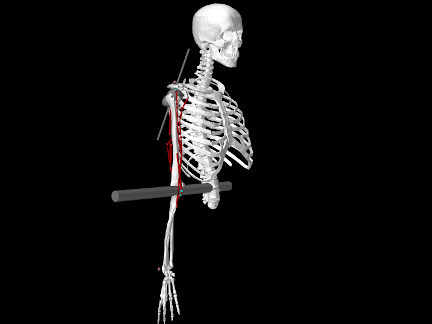
\includegraphics[]{images/OpenSimArm26} 
   \else 
      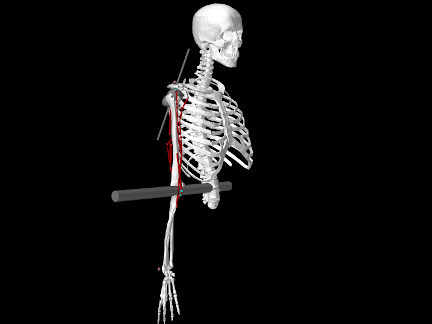
\includegraphics[width=3.75in]{images/OpenSimArm26} \fi
\end{center}
\caption{{\tt OpenSimArm26} loaded into ArtiSynth.}
\label{OpenSimArm26:fig}
\end{figure}
%
When loaded into ArtiSynth, the model appears as in Figure
\ref{OpenSimArm26:fig}. The OpenSim model contains a number of components that are {\it not} implemented
by ArtiSynth, as seen by the console messages
\begin{verbatim}
OpenSimParser: ignoring ControllerSet
OpenSimParser: ignoring ContactGeometrySet
OpenSimParser: ignoring ProbeSet
\end{verbatim}

After calling {\tt createModel()}, the {\tt build()} method changes the view
orientation, sets damping for the rigid bodies. and creates control panels to
adjust the excitations and joint coordinates. These are actions described
further in Section \ref{inspectingAndTuning:sec}.

\section{The component hierarchy}
\label{OpenSimHierarchy:sec}

{\tt OpenSimParser} arranges implementing components within {\tt MechModel} in a
manner that preserves the hierarchy and naming of the original OpenSim
model. This results in a component hierarchy different from the canonical one
used by {\tt MechModel}, in which components are placed in container lists by
type (e.g., particles in a {\tt PointList<Particle>} named {\tt "particles"},
rigid bodies in a {\tt RenderableComponentList<RigidBody>} named {\tt
"rigidBodies"}, axial springs in an {\tt AxialSpringList<AxialSpring>} list
named {\tt "axialSprings"}). However, as described in Section 
\ref{GeneralComponentArrangements:sec}, 
applications are free to create custom component arrangements, and {\tt
OpenSimParser} does this, recreating the basic OpenSim containers {\tt
"bodyset"}, {\tt "jointset"} (for OpenSim 4), {\tt "forceset"}, {\tt
"constraintset"} and {\tt "markerset"}. Figure \ref{Arm26Hierarchy1:fig}
illustrates this by showing the ArtiSynth navigation panel for the {\tt
OpenSimArm26} example. The only original {\tt MechModel} component that appears
is the {\tt collisionManager} (the other canonical containers, such as {\tt
"particles"}, {\tt "rigidBodies"}, etc., are still present, but don't appear
because they are empty).

\begin{figure}[ht]
\begin{center}
   \iflatexml 
      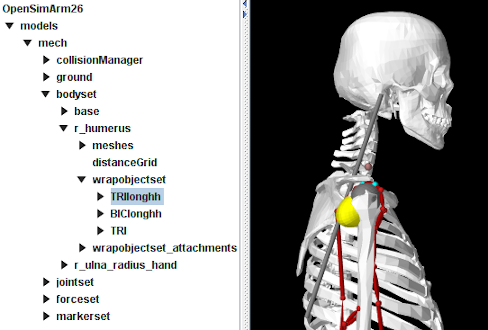
\includegraphics[]{images/Arm26Hierarchy1} 
   \else 
      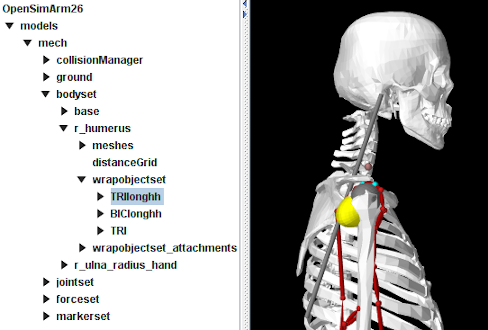
\includegraphics[width=3.75in]{images/Arm26Hierarchy1} \fi
\end{center}
\caption{Component hierarchy for {\tt OpenSimArm26}, showing
the body set in particular, with a wrap object selected.}
\label{Arm26Hierarchy1:fig}
\end{figure}

\subsection{Ground}

If present, the OpenSim 4 {\tt "ground"} component appears as its own
component, implemented using a \javaclass[\mech]{RigidBody} whose {\sf dynamic}
property is set {\tt false} and {\sf grounded} property is set {\tt true}.

\subsection{Body set}

The body set is implemented as a {\tt RenderableComponentList<RigidBody>}, with
each body implemented by a special implementation of
\javaclass[\mech]{RigidBody} that contains a
child component named {\tt "wrapobjectset"} that in turn contains any attached
wrap objects.  Wrap objects themselves are implemented by special instances
of \javaclass[\mech]{RigidBody} that implement the
\javaclass[\mech]{WrapComponent} interface.  Figure \ref{Arm26Hierarchy1:fig}
shows the navigation panel with the body {\tt r\_humerus} expanded and the wrap
object {\tt TRIlonghh} selected. Other body components include {\tt meshes} and
{\tt distancegrid}, which are defined for all ArtiSynth rigid bodies, and {\tt
wrapobjectset\_attachments}, which are the internal attachments connecting the
wrap objects to the body.

For OpenSim 3 models, each body also contains a child component {\tt "joint"},
containing the single joint for which that body is the parent. This is in place
of the joint set provided by OpenSim 4.

\subsection{Joint set}

For OpenSim 4, the joint set is implemented as a {\tt
RenderableComponentList<JointBase>} containing \javaclass[\mech]{JointBase}
components realizing the various OpenSim joints. Custom joints, in particular,
are implemented by \javaclass[\osim.customjoint]{OpenSimCustomJoint}.

\subsection{Force set}

\begin{figure}[ht]
\begin{center}
   \iflatexml 
      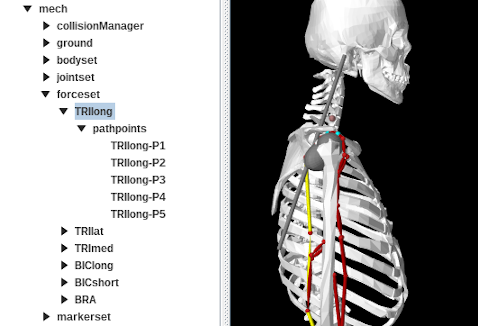
\includegraphics[]{images/Arm26Hierarchy2} 
   \else 
      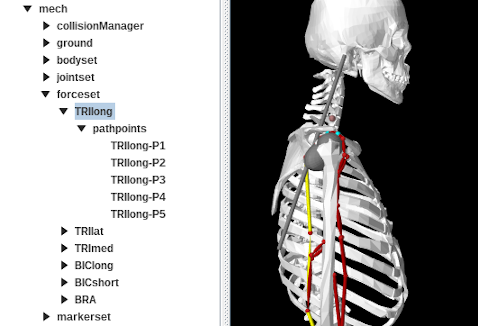
\includegraphics[width=3.75in]{images/Arm26Hierarchy2} \fi
\end{center}
\caption{Component hierarchy for {\tt OpenSimArm26}, showing the force set in
particular, with a muscle.}
\label{Arm26Hierarchy2:fig}
\end{figure}

The force set is implemented as a {\tt RenderableComponentList<ModelComponent>}
containing all the supported force effectors. Bushings and
CoordinateLimitForces are realized using \javaclass[\mech]{FrameSpring} and
\javaclass[\mech]{JointLimitForce}. Muscles and point-to-point springs are
implemented using a special implementation of
\javaclass[\mech]{MultiPointMuscle} that contains a child
component named {\tt "pathpoints"} that in turn contains all the muscle's path
points. Each path point is implemented as a {\tt FrameMarker} attached to one
of the bodies in the body set. Figure
\ref{Arm26Hierarchy2:fig} shows the navigation panel with the muscle {\tt
TRIlong} selected and also expanded to show the path points.

Currently supported OpenSim muscles include {\tt Thelen2003Muscle} and {\tt
Millard2012EquilibriumMuscle}, which are implemented using the {\tt
MultiPointMuscle} materials
\javaclass[\mats]{Thelen2003AxialMuscle} and 
\javaclass[\mats]{Millard2012AxialMuscle} 
(Section \ref{EquilibriumMuscleMaterials:sec}).
All other OpenSim muscles are implemented as a generic
instance of
\javaclass[\mats]{ConstantAxialMuscle}
(Section \ref{sec:mechii:musclematerials}) whose {\sf maxForce} property is set
to the specified {\tt max\_isometric\_force}.

\subsection{Constraint set}

The constraint set is implemented as a {\tt ComponentList<ConstrainerBase>}
containing all the supported constrainers. At present, these include {\tt
CoordinateCouplerConstraint} and {\tt PointConstraint}, realized by
\javaclass[\mech]{JointCoordinateCoupling} and
\javaclass[\mech]{SphericalJoint}, respectively.

\subsection{Marker set}

The marker set is implemented as a {\tt PointList<Marker>} with each marker
realized using \javaclass[\mech]{FrameMarker}.

\section{Inspecting and tuning the model}
\label{inspectingAndTuning:sec}

\subsection{Visualization}

\begin{figure}[ht]
\begin{center}
   \iflatexml 
      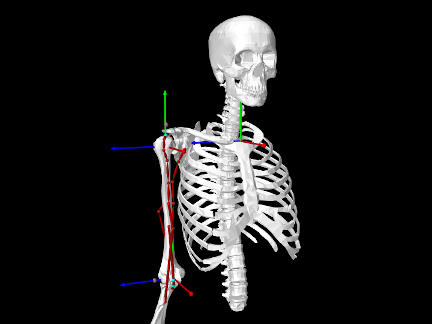
\includegraphics[]{images/Arm26BodyFrames} 
   \else 
      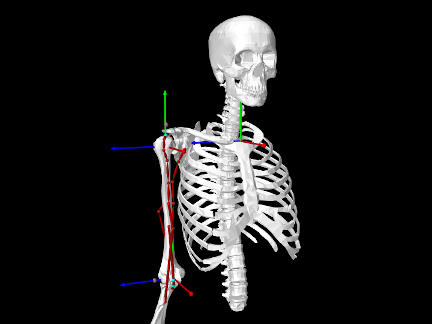
\includegraphics[width=3.75in]{images/Arm26BodyFrames} \fi
\end{center}
\caption{{\tt OpenSimArm26} with body coordinate frames visible.}
\label{Arm26BodyFrames:fig}
\end{figure}

ArtiSynth makes an attempt to preserve the visualization characteristics of the
original OpenSim model, but this is not guaranteed. The rendering and appearance
of all components can be customized, either interactively (as described under
``Editing Properties'' in the \artisynthManual{uiguide}{ArtiSynth User
Interface Guide}), or in code, as discussed in Section \ref{RenderProperties:sec}

The ``frame geometry'' associated with OpenSim bodies is not explicitly
supported, because ArtiSynth rigid bodies and frames already have a
visualization mechanism for their coordinate axes through their {\sf
axisLength} and {\sf axisDrawStyle} properties. The same is true for wrap
objects, which are realized as rigid bodies connected to their parent body via
a frame attachment.

{\tt OpenSimParser} does provide the following convenience methods to control
the visibility and coordinate frame rendering of bodies and wrap objects:
%
\begin{methodtable}{0.67}{0.33}
\midline
%
\methodentry
{\osim.OpenSimParser.setBodyFramesVisible(,)}%
{void setBodyFramesVisible (AxisDrawStyle style, double axisLen)}%
{Set axis rendering for bodies.}%
%
\methodentry
{\osim.OpenSimParser.setWrapObjectFramesVisible(,)}%
{void setWrapObjectFramesVisible (AxisDrawStyle style, double axisLen)}%
{Set axis rendering for wrap objects.}%
%
\methodentry
{\osim.OpenSimParser.setWrapObjectsVisible()}%
{void setWrapObjectsVisible (boolean visible)}%
{Set overall visibility of wrap objects.}%
%
\midline
\end{methodtable}
%
A method is supplied to control the collective visibility of wrap objects since
they are distributed among the bodies. (The collective visibility of
bodies, joints, forces, etc. can be controlled by setting the visibility of
the containers {\tt "bodyset"}, {\tt "jointset"}, {\tt "forceset"}, etc.)

Placing the following code at the end of the {\tt OpenSimArm26} example
causes the model to appear as in Figure \ref{Arm26BodyFrames:fig}:
%
\begin{lstlisting}[]
import maspack.render.Renderer.AxisDrawStyle;
...
   myParser.setWrapObjectsVisible(false);
   myParser.setBodyFramesVisible (AxisDrawStyle.ARROW, 0.12);
\end{lstlisting}
%

For observing the behavior of joints, it is often useful to display the axes
of their C and D coordinates frames. As described in Section
(\ref{RenderingJoints:sec}), this can be controlled by the joint properties
{\sf drawFrameC}, {\sf drawFrameD}, and {\sf axisLength}, which can be set
either in code or interactively (by selecting the joint and choosing {\sf Edit
properties ...} from the context menu).

Finally, the coordinate system for OpenSim models is usually arranged with the
$y$ axis vertical, whereas ArtiSynth defaults to the $z$ axis vertical.  While
{\tt OpenSimParser} will set gravity to whatever is specified in the OpenSim
file, the viewer orientation must be set by the application, using the root
model method {\tt setDefaultViewOrientation()}:
%
\begin{lstlisting}[]
import maspack.matrix.AxisAlignedRotation
...

   setDefaultViewOrientation (AxisAlignedRotation.X_Y);
\end{lstlisting}
%

\subsection{Interactive contol panels}
\label{OpenSimPanels:sec}

As discussed in Section \ref{ControlPanels:sec}, applications can create {\it
control panels} to interactively adjust the values of various component
properties. (Properties panels for one or more components can also be created
on demand by selecting the components then choosing {\sf Edit properties ...}
from the context menu.)

Also, as shown in the example {\tt OpenSimArm26}, {\tt OpenSimParser}
provides convenience methods to create two types of control panel:

\begin{itemize}

\item {\tt CoordinatePanel}s (Section \ref{CoordinatePanels:sec}) to
adjust joint coordinate values.

\item Control panels to adjust muscle excitations.

\end{itemize}

The methods are:
%
\begin{methodtable}{0.67}{0.33}
\midline
%
\methodentry
{\osim.OpenSimParser.createCoordinatePanel()}%
{CoordinatePanel createCoordinatePanel()}%
{Create panel for all coordinates.}%
%
\methodentry
{\osim.OpenSimParser.createCoordinatePanel(Collection)}%
{CoordinatePanel createCoordinatePanel (Collection<JointBase> joints)}%
{Create panel for specified joints.}%
%
\methodentry
{\osim.OpenSimParser.createCoordinatePanel(String)}%
{CoordinatePanel createCoordinatePanel (String[] coordNames)}%
{Create panel for named coordinates.}%
%
\methodspace{0.5em}%
\methodentry
{\osim.OpenSimParser.createExcitationPanel()}%
{ControlPanel createExcitationPanel ()}%
{Create panel for all muscles.}%
%
\methodentry
{\osim.OpenSimParser.createExcitationPanel(String)}%
{ControlPanel createExcitationPanel (String[] muscleNames)}%
{Create panel for named muscles.}%
%
\midline
\end{methodtable}
%
\begin{sideblock}
At present, {\tt CoordinatePanel}s do not support the adjustment of other
coordinate properties, such as locking or ranges. However, these can set in
code (Section \ref{coordinateLimitsAndLocking:sec}), and some
can also be set interactively by selecting the joint and
opening its property panel.
\end{sideblock}

\subsection{Model tuning}

We recommend testing the model by running it under forward simulation to ensure
that it behaves as expected. Some parameters, particularly those relative to
damping, may need to be adjusted.  There are several steps to this process.

\begin{itemize}

\item {\it Check joint function and damping}. Remove all force effectors and
let the model fall under gravity. If the body is not connected to ground,
select an appropriate body and set its {\sf dynamic} property to {\tt false}.
Force effectors can be removed by selecting the {\tt "forceset"} and choosing
{\sf Delete} in the context menu; this can also be done in code, as described
in Section \ref{OpenSimRemoving:sec}. 

\begin{sideblock}
With all force effectors removed, any model instability almost certainly
reflects a problem involving either bodies with zero inertia, or bodies that
are overconstrained. Both situations will result in a ``perturbed pivots''
message like the following appearing on the console output:
%
\begin{verbatim}
Pardiso: num perturbed pivots=3
\end{verbatim}
%
If this occurs, try to isolate the problem by selectively removing joints
and/or bodies. This can be done interactively by selecting them in the viewer
or navigation panel and choosing {\sf Delete} from the context menu.
Components can also be removed in code, as per
Section \ref{OpenSimRemoving:sec}.  Issues sometimes arise over the ``ground''
body, which OpenSim uses to represent ground (ArtiSynth does not require a
ground body). In OpenSim 3 models, where ground is not an explicit component,
one should ensure that its {\sf dynamic} property is set to {\tt false}.
\end{sideblock}

\begin{sideblock}
Stability issues may arise for bodies which are very small or can rotate quite
quickly. This can sometimes be addressed by specifying more damping (and
sometimes {\sf rotaryDamping} specifically) for these bodies. Alternatively,
one may wish to reduce the simulation step size, from the default of 0.01 sec
down to values around 0.001 or possibly lower. This can be interactively
adjusted in the GUI, and once a suitable value is found, set in code using the
root model's {\tt setMaxStepSizeMethod()}:
%
\begin{lstlisting}[]
   setMaxStepSize (0.001);
\end{lstlisting}
%
\end{sideblock}

In addition to gravity, you can also use the pull controller (see ``Pull
manipulation'' in the \artisynthManual{uiguide}{ArtiSynth User Interface
Guide}) to apply point forces to the various bodies. The main point of the
exercise is to see how the model behaves under gravity-like loads, and adjust
the damping parameters (Section \ref{BodyDamping:sec}) so that bodies come to
rest after an appropriate time. Critical, or slightly sub-critical, damping can
usually be achieved by setting the inertial damping for the {\tt MechModel} to
values in the range of 1-5, but sometimes one may want to adjust damping for
specific bodies, or also specify rotary or frame damping.

\begin{sideblock}
Damping in an ArtiSynth model is typically applied directly to its particles
and rigid bodies, and reflects the fact that body poses and velocities, instead
of joint coordinates and speeds, are the primary means of specifying the
model's dynamic state. OpenSim models often specify damping using {\tt
CoordinateLimitForces}; one may wish to remove or limit the use of those
components in ArtiSynth. Likewise, one may wish to reduce the use of damping in
the muscle forces.
\end{sideblock}

\item {\it Check the muscle wrapping}. Using a coordinate panel (Section
\ref{OpenSimPanels:sec}), adjust the coordinates and check that the muscle
wrapping appears correct. Issues that can sometimes arise include the path
failing to pass through small torus wrap objects, or not wrapping smoothly
around cylinders with radii due to insufficient knots in the wrap path.

Wrap path issues can usually be fixed by resetting the initialization points
and/or number of knots for the problematic wrap segments, using the methods
{\tt set/getNumKnots()} and {\tt set/getInitializingPoints()} described in
Section \ref{ObstacleWrapping:sec}. For example, the following
code might fix wrapping for a certain segment:
%
\begin{lstlisting}[]
  MultiPointSpring spr = (MultiPointSpring)myParser.findMuscle ("BIClong");
  int segIdx = 1;   // index of problematic segment
  Point3d xpnt;     // extra point to help initialize the wrap path
  ...
  spr.setNumKnots (segIdx, 30); // increase number of knots to 40
  spr.setInitializingPoints (   // reset initializing points
     segIdx, new Point3d[] { xpnt } ); 
  spr.updateWrapSegments();
\end{lstlisting}
%
The code makes use of the parser method {\tt findMuscle()},
described in Section \ref{OpenSimFindingComponents:sec}.

\item {\it Check quiescent and excited model behavior}. Start by checking the
behavior of the model with no loads or muscle excitations.  The purpose of this
exercise is to make sure that the model is stable in a ``rest''
state. Instability here will usually be the result of force effectors that are
generating forces that are too large for some reason. As when inspecting the
joint-body behavior, one should attempt to isolate the problem by selectively
removing components.

\begin{sideblock}
OpenSim muscles are sometimes configured with small non-zero initial
excitations, in order to facilitate the solution of muscle-tendon equilibrium.
ArtiSynth does not require this for its equilibrium muscle implementation, and
so applications are free to set muscle excitations to zero. {\tt OpenSimParser}
supplies the convenience method
\javamethod[\osim.OpenSimParser]{zeroMuscleExcitations()} for doing this.
\end{sideblock}

When forces are highly non-linear, stable model behavior may require reducing
the step size, as already described for body-joint calibration. It may also be
necessary to change the {\tt MechModel}'s {\sf stabilization} property from
{\tt GlobalMass} to {\tt GlobalStiffness}:
%
\begin{lstlisting}[]
import artisynth.core.mechmodels.MechSystemSolver.PosStabilization;
...
   myMech.setStabilization (PosStabilization.GlobalStiffness);
\end{lstlisting}
%
({\tt GlobalStiffness} is not the default setting because it increases
computation time).

\begin{sideblock}
A problem we have seen several times involves improper parameter settings for
OpenSim's {\tt CoordinateLimitForce} component, which is used to implement both
soft coordinate limits and coordinate damping. Rotational units for this
component are given in degrees (vs. radians for most other OpenSim components).
Modelers have sometimes not noticed this, leading to range limits that are
either far too small, or stiffness and damping values that are far too high.
\end{sideblock}

After checking the quiescent behavior, use a muscle excitation panel to check
that the model reacts as expected (and remains stable) when different muscles
are excited. In some cases, it may be desirable to adjust the muscle
parameters. For example, the rest lengths for a muscle implemented using {\tt
Millard2012AxialMuscle} could be adjusted as follows:
%
\begin{lstlisting}[]
import artisynth.core.materials.Millard2012AxialMuscle;
  ...
  double optl, tslack; // new opt fibre length and tendon slack length values
  ...
  // find problematic muscle
  MultiPointSpring spr = (MultiPointSpring)myParser.findMuscle ("BIClong");
  Millard2012AxialMuscle mmat = (Millard2012AxialMuscle)spr.getMaterial();
  // adjust the material
  mmat.setOptFibreLength (optl);
  mmat.setTendonSlackLength (tslack);
\end{lstlisting}
%
Another useful debugging technique can be to temporarily replace
the muscle material for problematic muscles with an instance of
\javaclass[\mats]{SimpleAxialMuscle} (Section \ref{SimpleAxialMuscle:sec}):
%
\begin{lstlisting}[]
  // replace material for problematic muscle
  MultiPointSpring spr = (MultiPointSpring)myParser.findMuscle ("BIClong");
  spr.setMaterial (new SimpleAxialMuscle (
     /*stiffness*/0, /*damping*/0, /*maxForce*/100));
\end{lstlisting}
%
If set with a given {\tt maxForce} and 0 stiffness and damping, a {\tt
SimpleAxialMuscle} material configures a muscle so that its tension is simply
equal to its {\sf excitation} times {\sf maxForce}.

\end{itemize}

\section{Model editing}
\label{OpenSimModelEditing:sec}

Once an OpenSim model has been imported into ArtiSynth and tuned, users will
typically want to modify it. This entails locating various OpenSim components,
which are then removed, modified or connected to other ArtiSynth components,
such as FEM models.

\subsection{Finding components}
\label{OpenSimFindingComponents:sec}

Locating the OpenSim components can done in several ways.  First, as with all
ArtiSynth models, any component that is a descendant of a container component
can be found by specifying its path name with respect to the container, using
\javamethod[\mbase.CompositeComponent]{findComponent()} method. For example,
the {\tt MultiPointMuscle} {\tt TRIlong} seen Figure \ref{Arm26Hierarchy2:fig}
could be obtained using
%
\begin{lstlisting}[]
import artisynth.core.mechmodel.MultiPointMuscle;
...

   MultiPointMuscle muscle = (MultiPointMuscle)mech.findComponent (
      "forceset/TRIlong/TRIlong");
\end{lstlisting}
%
where we know a priori that the sought component is a {\tt MultiPointMuscle} and
so are comfortable casting it to such. Likewise, the immediate children
of any composite component can be accessed using 
\javamethodAlt{\mbase.CompositeComponent.get(int)}{get(idx)} or
\javamethodAlt{\mbase.CompositeComponent.get(String)}{get(name)}.

Second, most ArtiSynth container classes implement the {\tt java.util}
interfaces {\tt Collection<C>} and {\tt Iterable<C>} with respect to their
component type {\tt C}, making list iteration easy:
%
\begin{lstlisting}[]
import artisynth.core.modelbase.RenderableComponentList;
import artisynth.core.mechmodels.RigidBody;
...

   // search the body set for a rigid body:
   RenderableComponentList<RigidBody> bodyset =
      (RenderableComponentList)mech.findComponent ("bodyset");
   for (RigidBody body : bodyset) {
      if (body.getName().equals ("r_humerus")) {
         System.out.println ("Found it!");
      }
   }
\end{lstlisting}
%
Finally, {\tt OpenSimParser} provides a number of methods for finding
components after the model has been created:

%
\begin{methodtable}{0.65}{0.35}
\midline
%
\methodentry
{\osim.OpenSimParser.getGround()}%
{RigidBody getGround()}%
{Returns ground, if present.}%
%
\methodentry
{\osim.OpenSimParser.getBodySet()}%
{RenderableComponentList<RigidBody> getBodySet()}%
{Returns the body set.}%
%
\methodentry
{\osim.OpenSimParser.findBody()}%
{RigidBody findBody (String name)}%
{Finds a body by name.}%
%
\methodspace{0.5em}%
\methodentry
{\osim.OpenSimParser.getWrapObjects()}%
{ArrayList<WrapComponent> getWrapObjects() }%
{Returns a list of all wrap objects.}%
%
\methodentry
{\osim.OpenSimParser.findWrapObject()}%
{WrapComponent findWrapObject (String name) }%
{Finds a wrap object by name.}%
%
\methodentry
{\osim.OpenSimParser.getBodyWrapObjects()}%
{ArrayList<WrapComponent> getBodyWrapObjects (RigidBody body)}%
{Returns all wrap objects for a body.}%
%
\methodentry
{\osim.OpenSimParser.getMuscleWrapObjects()}%
{List<WrapComponent> getMuscleWrapObjects (\brh PointSpringBase muscle)}%
{Returns all wrap objects for a muscle.}%
%
\methodspace{0.5em}%
\methodentry
{\osim.OpenSimParser.getJointSet()}%
{RenderableComponentList<JointBase> getJointSet()}%
{Returns the joint set.}%
%
\methodentry
{\osim.OpenSimParser.getJoints()}%
{ArrayList<JointBase> getJoints()}%
{Returns a list of all the joints.}%
%
\methodentry
{\osim.OpenSimParser.findJoint()}%
{JointBase findJoint (String name)}%
{Finds a joint by name.}%
%
\methodentry
{\osim.OpenSimParser.getCoordinates()}%
{ArrayList<JointCoordinateHandle> getCoordinates()}%
{Returns a list of all coordinates.}%
\methodentry
{\osim.OpenSimParser.findCoordinate()}%
{JointCoordinateHandle findCoordinate (String name)}%
{Finds a coordinate by name.}%
%
\methodspace{0.5em}%
\methodentry
{\osim.OpenSimParser.getForceSet()}%
{RenderableComponentList<ModelComponent> getForceSet()}%
{Returns the force set.}%
\methodentry
{\osim.OpenSimParser.getForceComponents()}%
{ArrayList<ForceComponent> getForceComponents()}%
{Returns all force components.}%
%
\methodentry
{\osim.OpenSimParser.getMusclesAndSprings()}%
{ArrayList<PointSpringBase> getMusclesAndSprings()}%
{Returns all muscles and axial springs.}%
%
\methodentry
{\osim.OpenSimParser.getMuscles()}%
{ArrayList<MuscleComponent> getMuscles()}%
{Returns all muscles.}%
%
\methodentry
{\osim.OpenSimParser.findForceComponent()}%
{ForceComponent findForceComponent (String name)}%
{Finds a force component by name.}%
%
\methodentry
{\osim.OpenSimParser.findMuscleOrSpring()}%
{PointSpringBase findMuscleOrSpring (String name)}%
{Finds muscle or axial spring by name.}%
%
\methodentry
{\osim.OpenSimParser.findMuscle()}%
{MuscleComponent findMuscle (String name)}%
{Finds muscle by name.}%
%
\methodspace{0.5em}%
\methodentry
{\osim.OpenSimParser.getConstraintSet()}%
{RenderableComponentList<ConstrainerBase> getConstraintSet()}%
{Returns the constraint set.}%
%
\methodentry
{\osim.OpenSimParser.findConstraint()}%
{ConstrainerBase findConstraint (String name)}%
{Finds a constraint by name.}%
%
\methodspace{0.5em}%
\methodentry
{\osim.OpenSimParser.getMarkerSet()}%
{PointList<Marker> getMarkerSet()}%
{Returns the marker set.}%
%
\methodentry
{\osim.OpenSimParser.findMarker()}%
{Marker findMarker (String name)}%
{Finds a marker by name.}%
%
%
%\methodspace{0.5em}%
%\brh
\midline
\end{methodtable}
%
%
The following should be noted about these methods:

\begin{itemize}

\item For OpenSim 3 models, {\tt getGround()} and {\tt getJointSet()} will both
return {\tt null}. To obtain a list of all joints in this case, one can use
{\tt getJoints()}, which collects all joints regardless of where they are
located within the hierarchy.

\item Access to joint coordinates is provided by means of a 
\javaclass[\mech]{JointCoordinateHandle}, which encapsulates
the information about both the coordinate and the joint to which it belongs.

\item The muscles and axial spring components returned by {\tt
getMusclesAndSprings()} are a subset of the components returned by {\tt
getForceComponents()}.

\end{itemize}

\subsection{Removing components}
\label{OpenSimRemoving:sec}

For component removal, most container classes supply {\tt remove()} methods
that allow this to be done directly. However, care must be be taken that other
model components either do not have a hard dependency on those being removed,
or that the dependent components are be removed as well.  For example, any
muscle component has a hard dependency on the frame markers that serve as its
origin and insertion points, so removing either of these markers necessitates
removing the muscle as well. The easiest way to ensure the removal of
one or more components {\it and} their dependencies is to use the utility methods
%
\begin{methodtable}{0.98}{0.02}
\midline
%
\methodentry
{\mbase.ComponentUtils.deleteComponentAndDependencies()}%
{void ComponentUtils.deleteComponentAndDependencies (ModelComponent comp)}%
{\ }%
%
\methodspace{0.5em}%
\methodentry
{\mbase.ComponentUtils.deleteComponentsAndDependencies()}%
{void ComponentUtils.deleteComponentsAndDependencies (%
Collection<? extends ModelComponent> comps)}%
{\ }%
\midline
\end{methodtable}
%
For example, to remove a frame marker, one may call
%
\begin{lstlisting}[]
import artisynth.core.modelbase.ComponentUtils;
import artisynth.core.mechmodels.Marker;
...

   Marker mkr;
   
   ... locate the marker to remove ...

   ComponentUtils.deleteComponentAndDependencies (mkr);
\end{lstlisting}
%
In addition to removing components with hard dependencies, these methods also
take care of {\it soft} dependencies, by which some components adjust
themselves if certain components are deleted. For example, a {\tt
MultiPointMuscle} has a soft dependency on any wrap object that it references:
if the wrap object is removed, the muscle deletes its internal
reference to the object and update its wrap path.

\begin{sideblock}
Use of these methods is equivalent to invoking the {\tt Delete} operation from
the context menu in the ArtiSynth GUI, which also looks for dependent
components and queries the user for confirmation if any are found (Figure
\ref{deletingMarkerInGui:fig}).
\end{sideblock}

\begin{figure}[ht]
\begin{center}
   \iflatexml 
      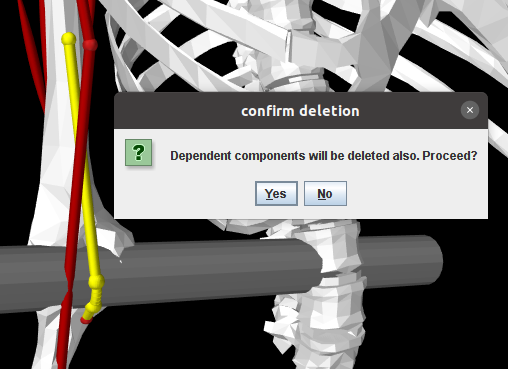
\includegraphics[]{images/deletingMarkerInGui} 
   \else 
      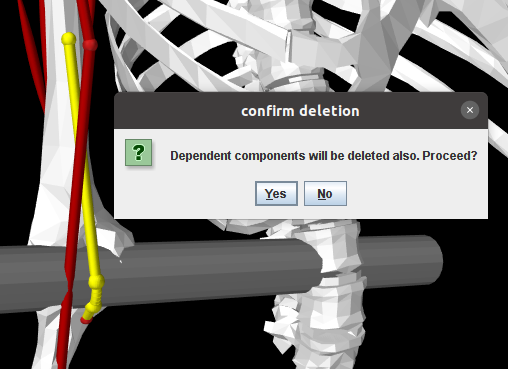
\includegraphics[width=3.75in]{images/deletingMarkerInGui} 
   \fi
\end{center}
\caption{Using the GUI to delete a marker that serves as a muscle origin
triggers a warning that other components (in this case the muscle) will also be
deleted.}
\label{deletingMarkerInGui:fig}
\end{figure}

There {\it are} situations where one may wish to remove a component but {\it
not} the components that depend on it. For example, if one wishes to replace a
rigid body with a different rigid body, or an FEM model of the same structure,
one may wish to transfer to the new body the joints and markers that depend on
the original body. This is described more in the following section.

\subsection{Attaching and transferring to ArtiSynth components}
\label{OpenSimAttaching:sec}

New ArtiSynth components can be attached to OpenSim components through the
general point and frame attachment mechanisms described in Sections
\ref{Attachments:sec}, \ref{sec:fem:nodeattachments}, and
\ref{sec:fem:frameattachments}.

Contact behaviors (Chapter \ref{ContactAndCollision:sec}) can also be set
between OpenSim and/or ArtiSynth components. When working with the former, it
may be desirable to replace body surface meshes
(using \javamethod[\mech.RigidBody]{setSurfaceMesh()}), or add additional
meshes for collision purposes (using \javamethod[\mech.RigidBody]{addMesh()}).

In some instances, one may wish to transfer OpenSim joints, path points,
markers or wrap objects to new ArtiSynth components.  For joints, one can use
the various {\tt setBodies()} or {\tt setBodyA/B()} methods described in
Section \ref{CreatingJoints:sec} to reassign one or both bodies for an existing
joint. 

OpenSim wrap objects are attached to their parent bodies using a frame
attachment. Attaching to a different body involves replacing this
attachment. However, when doing so, the existing frame attachment must be
removed and the existing wrap object should {\it probably} be removed from its
parent body and placed elsewhere in the component hierarchy. To make this
easier, {\tt OpenSimParser} supplies the method
\javamethod[\osim.OpenSimParser]{removeWrapObject()} that disconnects a wrap
object from its parent body and removes its attachment; the application can
then move the wrap object elsewhere and reattach it:
%
\begin{lstlisting}[]
  MechModel mech;       // mech model containing everything
  OpenSimParser parser; // parser that imported the model
  WrapComponent wobj;   // wrap object to be reassigned
  RigidBody newBody;    // new body to connect wobj to
  ...
  parser.removeWrapObject(wobj);     // detach wobj and remove its attachment
  RigidBody wbody = (RigidBody)wobj; // wrap objects are also rigid bodies
  mech.addRigidBody (wbody);         // move wobj to standard body list
  mech.attachFrame (wbody, newBody); // attach to new body
\end{lstlisting}
%

For transferring markers and path points to other bodies, {\tt OpenSimParser}
supplies the methods
%
\begin{methodtable}{0.9}{0.1}
\midline
%
\methodentry
{\osim.OpenSimParser.replacePathPoint(,,)}%
{Marker replacePathPoint (PointSpringBase muscle, Marker pnt,
PointAttachable body)}%
{\ }%
%
\methodspace{0.5em}
\methodentry
{\osim.OpenSimParser.replaceMarker(,)}%
{Marker replaceMarker (Marker mkr, PointAttachable body)}%
{\ }%
%
\midline
\end{methodtable}
%
{\tt replacePathPoint()} replaces the path point {\tt pnt} of the specified
{\tt muscle} with a {\it new} point (also implemented as a {\tt Marker},
though not necessarily a {\tt FrameMarker}) attached to the specified {\tt
body}. The new point is placed in the same location of the muscle as the
original. Similarly, {\tt replaceMarker()} replaces the marker {\tt mkr} within
the marker set with a new marker attached to the specified {\tt body}.

\subsection{Example: replacing the elbow joint with a contact FEM model}
\label{Arm26FemElbow:sec}

\begin{figure}[ht]
\begin{center}
   \iflatexml 
      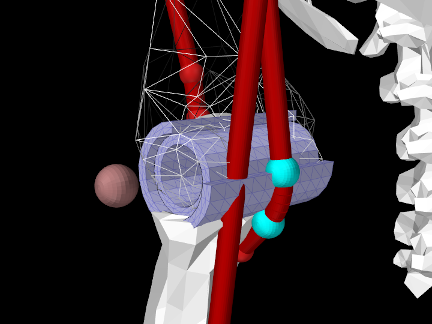
\includegraphics[]{images/Arm26FemElbow} 
   \else 
      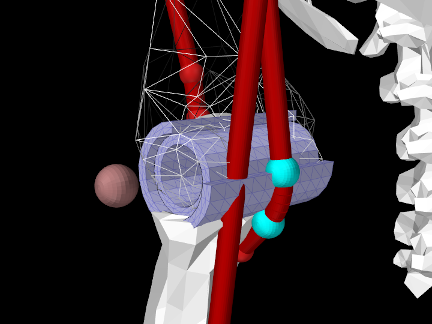
\includegraphics[width=3.75in]{images/Arm26FemElbow} 
   \fi
\end{center}
\caption{{\tt Arm26FemElbow} model, showing a closeup of the
toy FEM model used to emulate the elbow, with the humerus displayed as a
wireframe for greater visibility.}
\label{Arm26FemElbow:fig}
\end{figure}

The model 
\begin{verbatim}
  artisynth.demos.opensim.Arm26FemElbow
\end{verbatim}
presents a modified version of {\tt OpenSimArm26} in which the elbow joint has
been removed and replaced with a (very simple) contact model involving two
nested FEM cylinders simulating cartilage layers, with the outer layer
attached to the lower arm and the inner one attached to the humerus (Figure
\ref{Arm26FemElbow:fig}). Additional stability is supplied by a
\javaclass[\mech]{FrameSpring}, located where the elbow joint was, that
prevents sliding and limits rotation along and about the joint axis. The class
definition, excluding {\tt import} statements, is shown below:
%
\lstset{numbers=left} 
\iflatexml
%% Hack: latexml lstinputlisting doesn't handle firstline correctly
\lstset{firstnumber={-26}}
\lstinputlisting[firstline=1]{../../src/artisynth/demos/opensim/Arm26FemElbow.java}
\lstset{firstnumber={1}}
\else
\lstinputlisting[firstline=28]{../../src/artisynth/demos/opensim/Arm26FemElbow.java}
\fi
\lstset{numbers=none}
In the {\tt build()} method, {\tt super.build()} is first called to create the
{\tt OpenSimArm26} model which this example extends. Then the geometry folder is
located relative to the model's source folder (line 25), and the humerus, lower
arm, and elbow components are located using the parser's {\tt findBody()} and
{\tt findJoint()} methods (lines 25-30).

The FEM models used to simulate the inner and outer cartilage layers are
defined with respect to the elbow's D frame, which is located in world
coordinates using its {\tt getCurrentTDW()} method (line 35).  The models
themselves, which are defined as Gmsh files in the geometry folder, are read
using {\tt GmshReader} (Section \ref{FemGeometryFiles:sec}), initialized with
the helper method {\tt initializeFem()} which sets their material and rendering
properties (lines 5-19), transformed to the D frame, and added to the {\tt
MechModel} (lines 40-48). The inner and outer layers are then connected to the
humerus and lower arm, respectively, by attaching nodes whose numbers are
specified by node number files (Section \ref{SelectingNodesInViewer:sec})
also located in the geometry folder (lines 52-60).

With the cartilage models connected, the elbow joint is removed (line 64).  It
is replaced by a {\tt FrameSpring} (lines 65-74) to supply the stabilization
effected by other tissues surrounding the joint. The spring is centered on the
D frame, and uses a {\tt PowerFrameMaterial}
(Section \ref{PowerFrameMaterial:sec}) with all stiffnesses set to 0 except for
a translational stiffness along $z$ to limit sliding along the joint axis, and
a rotational stiffness (with a deadband of $\pi$) about $z$ to limit joint axis
rotation to the approximate range $[0, \pi]$.

\begin{sideblock}
Note the use of {\tt setUseTransformDC(false)} when setting up the {\tt
FrameSpring}. As described in Section \ref{FrameSpringCoordinateFrames:sec},
this makes the spring compute its restoring forces using $\T_{CD}$, which is
the same displacement used by joints, instead of its inverse $\T_{DC}$.  This
in turn means that translations and rotations will have the same directionality
in the spring as in the original joint.
\end{sideblock}

Frictionless contact is enabled between the cartilage models (lines 77-78), and
to improve stability this contact is made compliant
(Section \ref{CompliantContact:sec}, lines 80-82) and the model's step size is
decreased to 0.005 sec (line 83).

Removal of the elbow joint revealed that the quiescent forces in the muscles
{\tt "BIClong"} and {\tt "BRA"} were large enough to cause a large upward
impulse at the start of the simulation. To eliminate this, the tendon slack
length for these muscles is reset to equal the difference between the total
muscle length and the optimal fibre length (lines 87-91; this calculation uses
the fact that the optimal pennation angle is 0). To further reduce initial
forces, the bias excitations present in the OpenSim model are also removed
(line 93). Finally, to enable the FEM joint to be seen, the wrap object {\tt
"TRI"} is made invisible (line 96).

To run this example in ArtiSynth, select {\sf All demos > opensim >
Arm26FemElbow} from the {\sf Models} menu.

\begin{sideblock}
It is possible to make this model go unstable, usually with an ``inverted
elements'' error, if sufficiently large or abrupt forces are exerted on it via
the pull controller or the excitation panel.
\end{sideblock}

\subsection{Example: replacing the humerus with a FEM model}
\label{Arm26FemHumerus:sec}

\begin{figure}[ht]
\begin{center}
   \iflatexml 
      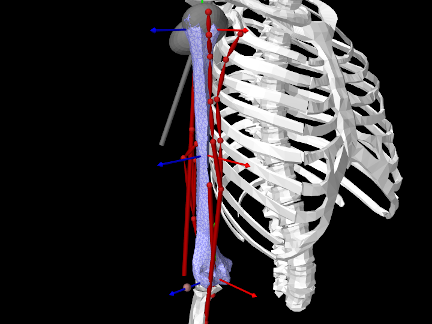
\includegraphics[]{images/Arm26FemHumerus} 
   \else 
      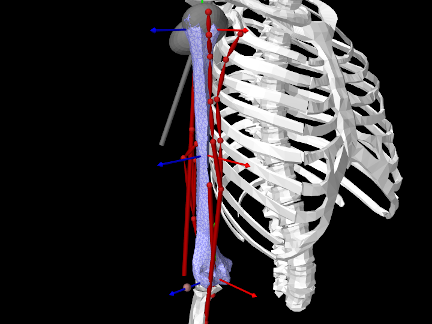
\includegraphics[width=3.75in]{images/Arm26FemHumerus} 
   \fi
\end{center}
\caption{{\tt Arm26FemHumerus} model, showing the FEM humerus
and the three coordinate frames embedded into its top, middle and bottom.}
\label{Arm26FemHumerus:fig}
\end{figure}

The model 
\begin{verbatim}
  artisynth.demos.opensim.Arm26FemHumerus
\end{verbatim}
presents a modified version of {\tt OpenSimArm26} in which the humerus has been
replaced with an FEM model, with the joints, wrap objects, and muscle path
points transferred from the humerus body to the FEM model
(Figure \ref{Arm26FemHumerus:fig}). Most of this transfer is based on
three \javaclass[\mech]{Frame} objects that are attached to the top, middle and
center of the FEM model, using the methods described in Section
\ref{sec:fem:frameattachments}. These frames serve as anchors for attaching the
shoulder and elbow joints, the wrap objects, and the muscle path points that
are far enough from the FEM that direct point-to-FEM connections are
problematic. Forces applied to wrap objects and path points are transmitted to
the FEM model via the frames, which are given a large number of supporting
nodes so that the resulting stresses are distributed across a reasonable number
of elements.

The {\tt build()} method for {\tt Arm26FemHumerus} makes use of the following
helper methods:
%
\lstset{numbers=left} 
\iflatexml
%% Hack: latexml lstinputlisting doesn't handle firstline correctly
%\lstset{firstnumber={-25}}
\lstinputlisting[firstline=131,lastline=180]{../../src/artisynth/demos/opensim/Arm26FemHumerus.java}
%\lstset{firstnumber={1}}
\else
\lstset{firstnumber={131}}
\lstinputlisting[firstline=131,lastline=180]{../../src/artisynth/demos/opensim/Arm26FemHumerus.java}
\lstset{firstnumber={1}}
\fi
\lstset{numbers=none}

{\tt nearestFrame()} finds the frame whose origin is nearest to a given
position vector. {\tt createFrameAttachment()} creates a {\tt
FrameFem3dAttacment} (Section \ref{sec:fem:frameattachments}) for a frame
located at the pose described by {\tt TFW} and supported by a set of nodes that
are within a prescribed distance of the frame's $z$ axis.  This choice of
supporting nodes is based on the fact that much of the force in this model
involves moments about the $z$ axis, but other choices are possible.  The
critical point is to choose enough nodes so that stresses induced frame forces
are distributed reasonably well within the model. The method {\tt
addFemFrame()} creates a \javaclass[\mech]{Frame} object initially located at
{\tt TFW}, gives it a {\tt name}, and attaches it to a FEM model using an
attachment created by {\tt createFrameAttachment()}.

The {\tt build()} method itself is listed below:
%
\lstset{numbers=left} 
\iflatexml
%% Hack: latexml lstinputlisting doesn't handle firstline correctly
%\lstset{firstnumber={-25}}
\lstinputlisting[firstline=40,lastline=128]{../../src/artisynth/demos/opensim/Arm26FemHumerus.java}
%\lstset{firstnumber={1}}
\else
\lstset{firstnumber={40}}
\lstinputlisting[firstline=40,lastline=128]{../../src/artisynth/demos/opensim/Arm26FemHumerus.java}
\lstset{firstnumber={1}}
\fi
\lstset{numbers=none}
%
First, {\tt super.build()} is called to create the {\tt OpenSimArm26} model
which this example extends. The parser's {\tt findBody()} method is then used
to locate the humerus body that is being replaced (line 45).

The FEM model replacing the humerus body is created and added to the {\tt
MechModel} at lines (47-66). A tetrahedral element mesh is created from a
surface mesh (read from a {\tt geometry} directory) by {\tt
FemFactory.createFromMesh()}. Material properties are assigned, with the FEM
model given the same density as that of the humerus body (which is higher than
bone density to account for the mass of surrounding tissue). Since the defining
surface mesh uses the same coordinate system as the original humerus mesh, the
model geometry can be transformed into the correct position using the pose of
the humerus body (line 59).

The remainder of the {\tt build()} method transfers the joints, wrap objects,
muscle path points and markers from the humerus body to the FEM model.  Joints
are transferred at lines 60-76. The humerus corresponds to body A of the
shoulder joint and body B of the elbow joint, and so {\tt setBodyA()} and {\tt
setBodyB()} are used, respectively, to reconnect these to the FEM model at the
shoulder's C frame and the elbow's D frame.  Attachments are generated by {\tt
createFrameAttachment()}, using the world locations of the C and D frames
returned by the joint methods {\tt getCurrentTCW()} and {\tt getCurrentTDW()}.

At lines 81-88, {\tt addFemFrame()} is used to create and attach three
anchoring frames to the top, middle and bottom of the FEM model. The top and
bottom frames are located the C and D frames of the shoulder and elbow joints,
while the middle frame is placed at an offset from the C frame. All wrap
objects connected to the humerus body are reconnected to one of these frames
(lines 91-100). For each wrap object, the parser's {\tt removeWrapObject()}
removes it from the OpenSim component hierarchy and deletes its attachment, the
object is cast to a {\tt RigidBody} and added to the {\tt MechModel}'s default
rigid body list (other locations could be used), and a new attachment is
created between the wrap object and the nearest anchor frame.

The muscle path points are transferred at lines 104-123. The code iterates
through all the points of all the muscles. Since {\tt OpenSimParser} implements
all path points as {\tt FrameMarker}s, each point can be cast to a {\tt
FrameMarker} and inspected to see if its frame is the original humerus body. If
it is, the point must be replaced with a new marker attached to the FEM model.
If the point is either the first or last path point, then it is an origin or
insertion and so is near enough to the FEM model than it can be attached
directly. Otherwise, it is attached to the nearest anchor frame. Point
replacement is performed by the parser's {\tt replacePathPoint()} method.

Lastly, the {\tt "r\_humerus\_epicondyle"} marker is transferred to the bottom
anchor frame, using the parser's {\tt replaceMarker()} method, and the humerus
body is removed from the body set. There is no need to do this removal using
the {\tt ComponentUtils} method {\tt deleteComponentAndDependencies()} since
all dependencies have been removed by the preceding steps.

To run this example in ArtiSynth, select {\sf All demos > opensim >
Arm26FemHumerus} from the {\sf Models} menu.

\ifdefined\maindoc
\else
\end{document}
\fi
